\documentclass[10pt,twocolumn,letterpaper]{article}
%% HSBDC2026

%% Language and font encodings
\usepackage[english]{babel}
\usepackage[utf8x]{inputenc}
\usepackage[T1]{fontenc}
\usepackage{caption,subcaption,graphicx,underscore,booktabs,titling}

\newcommand{\rowcmidrule}[1]{\cmidrule(lr){1-#1}}

%% Sets page size and margins
\usepackage[a4paper,top=3cm,bottom=2cm,left=3cm,right=3cm,marginparwidth=1.75cm]{geometry}

%% Useful packages
\usepackage{amsmath}
\usepackage{graphicx}
\usepackage[colorinlistoftodos]{todonotes}
\usepackage[colorlinks=true, allcolors=blue]{hyperref}
\usepackage{natbib}
\bibliographystyle{unsrt}
%% Title
\title{
		\usefont{OT1}{bch}{b}{n}
		\normalfont \normalsize \textsc{STEM Fellowship 2025-2026 High School Big Data Challenge} \\ [10pt]
		\huge From Harvest to Food Security: Machine Learning Forecasts for the United States\\
}
\selectlanguage{english}
\usepackage{authblk}
\author[1, 2]{Cathy Rong\thanks{Corresponding author: \href{mailto:cathyrong11@gmail.com}{cathyrong11@gmail.com}}}
\author[1]{Safiya Taher}
\author[1]{Sabrina Qian}
\author[1]{Renisa Ghosh}
\author[1]{Arthur Jiang}
\affil[1]{Old Scona Academic, Edmonton, Alberta, Canada}
\affil[2]{United World Colleges Red Cross Nordic, Flekke, Vestland, Norway}
\date{January 9, 2026}
\setlength {\marginparwidth }{2cm}

\newcommand{\WordCountfootnote}{
\begingroup
\renewcommand\thefootnote{}
\footnote{\textit{Word Count (excluding figures, tables, references, and title page):} 2854}
\addtocounter{footnote}{-1}
\endgroup
}

\begin{document}

\maketitle

\begin{abstract}
Food insecurity persists even in high-output agricultural systems, underscoring the need for timely national indicators. This study tests whether U.S. agricultural production signals can predict changes in a composite Food Security Index ($FSI$) using annual data (1970-2023) integrating USDA NASS QuickStats measures for three major staple crops: corn, soybeans, and wheat (yield, production, and area harvested) as well as engineering shock and lag features.

The prediction target expresses changes in a $FSI$ scaled from $[0,1]$ (higher = more food secure) constructed from four national indicators, including FAOSTAT supply/production measures and macro-climate variables: Food production index, Dietary energy supply, GDP per capita, and Temperature change on land. We first used regression models (Random Forest, RidgeCV, and Gradient Boosting) trained on 1970-2012 and tested on 2013-2023 data to predict annual changes in food security, $(\Delta FSI(t))$, evaluating accuracy with RMSE/MAE/ $R^2$ against a persistence baseline $FSI(t-1)$, and then converted $(\Delta FSI)$ into a binary direction label (positive $(>0)$, negative $(\le 0)$) to assess how well the same models predict year-to-year improvement vs decline using balanced accuracy.

Overall, results showed that the national crop statistics contain measurable predictive indicators for annual food security dynamics and motive extensions.

\end{abstract}  
{\textbf{Keywords}: \\ 
Agriculture, Food Security Index (FSI), Common Crop Indicators, Machine Learning}\WordCountfootnote

\section{Introduction}

Food insecurity persists even in highly productive agricultural systems because national food security depends on more than total crop output \cite{Long2020}. It depends on accessibility to safe, sufficient, and nutritious food while the system remains resilient to shocks \cite{Kavallari2014}. With climate variability \cite{Beach2010}, market disruptions \cite{Barnichon2022}, and economic pressures increasingly interacting, there is growing demand for timely, interpretable national indicators that can be tracked consistently over long periods to support policy \cite{Hatfield2011}.

Agricultural production is a consistently measured national variable. In the United States (U.S.), corn, soybeans, and wheat are well documented because they dominate staple crop production and shape downstream food and feed markets \cite{WinnePeersman2016, Kreitzman2020}. Annual changes in yields, acreage, and output reflect biophysical constraints and land-use responses. However, production alone does not represent national food security outcomes: access and affordability \cite{Manap2019}, supply chains \cite{Nava2023, Smith2007}, and broader macro conditions also introduce nonlinearities.

Researchers have previously developed composite food-security indicators to capture food security's multiple dimensions. The Global Food Security Index (GFSI) \cite{GFSI2022, akinniyi2024}, for example, assesses 113 countries across affordability, availability, quality and safety, and sustainability/adaptation, providing a transparent basis for policy analysis \cite{Bibi2023, Salles-Costa2022}. Inspired by these, we developed a U.S.-focused composite Food Security Index ($FSI$) using four indicators from Food and Agriculture Organization of the UN's corporate statistical database (FAOSTAT) \cite{FAOSTATindicator}: Food Production Index (domestic supply availability) \cite{NUBE20011275}, Dietary energy supply (dietary adequacy/quality) \cite{Henchion2017}, GDP per capita (economic access/affordability) \cite{Warr2014}, and Temperature on land change (sustainability stress) \cite{Bozkurt2021}.

We then forecasted $\Delta FSI$ using crop data from United States Department of Agriculture (USDA) National Agricultural Statistics Service (NASS) QuickStats \cite{USDANASS_QuickStats} combined with exogenous economic and price data from the U.S. Bureau of Labor Statistics (BLS) \cite{Varshita2024} and the World Bank (WB) \cite{worldbank2015, worldbank2025}. By cleaning, normalizing, and synthesizing these datasets, we trained and tested various machine learning models using multi-year data, with attention to directional annual changes ($\Delta FSI$). Results indicate that a trained Random Forest model provides the most accurate tracking of U.S. food security dynamics.

\section{Materials \& Methods}

\subsection{Data and Study Design}

\begin{figure*}
    \centering
    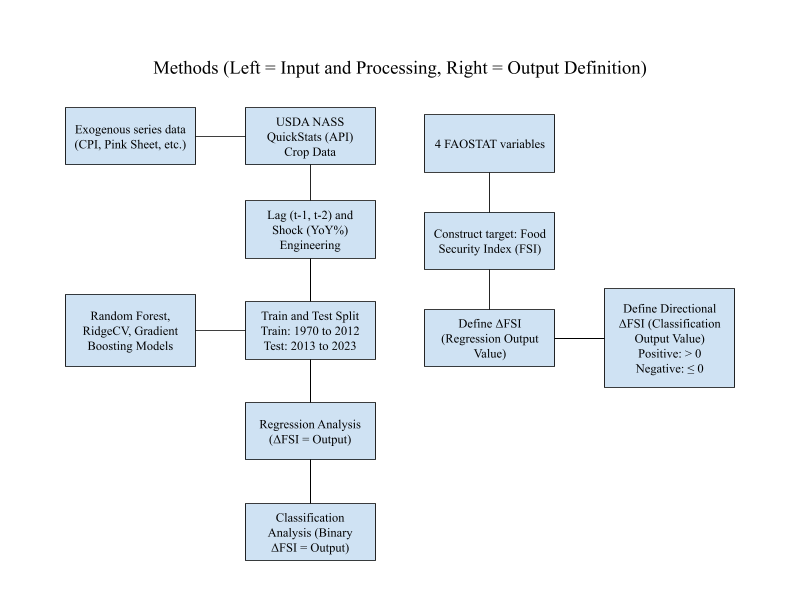
\includegraphics[width=1\linewidth]{fig1_flow_chart.png}
    \caption{Study Flow Chart}
    \label{fig:1}
\end{figure*}

We examine whether U.S. staple-crop production predicts changes in a composite Food Security Index ($FSI$) using annual data from 1970-2023 \cite{justin_oh_2023, owidagriprod}. Crop predictors (yield, total production, and harvested area) were obtained from USDA QuickStats for corn, soybeans, and wheat (N=1,944). The primary outcome is to define ($\Delta FSI$) as yearly change, where higher values indicate improving food security.

In addition, we included exogenous variables: food Consumer Price Index (CPI), its annual change from BLS, WB “Pink Sheet” indices (Energy, Agriculture, Food, Grains, Fertilizers, Metals \& Minerals), selected commodity prices (crude oil, maize, soybeans, and wheat with both Hard Red Winter and Soft Red Winter) and population data. All datasets were restricted to the U.S., aggregated to annual values, and merged by year into a master table; non-numeric entries were considered missing and dropped. To reduce bias and prevent leakage, we excluded state-level QuickStats variables so that training and evaluation reflect a national context.

The resulting dataset was then used for feature engineering (lags and year-over-year “shock” variables) and model evaluation using time-dependent training/testing splits. Multiple machine learning models were employed and trained to forecast $FSI$ dynamics. Model performance and sensitivity were assessed.

Figure \ref{fig:1} summarizes the end-to-end flow (data integration through validation). 

\subsection{Data Preparation}
Crop data retrieved from the USDA NASS QuickStats API \cite{USDANASS_QuickStats} using U.S.-level annual queries executed in Python (\texttt{requests}), were outputted as structured CSVs. Exogenous inputs (BLS food CPI, WB “Pink Sheet” indices/ prices, and population totals) were downloaded from their respective sources and integrated.

All preprocessing was performed in Python \cite{python11} using \texttt{pandas} \cite{pandas_reback2020} and \texttt{NumPy} \cite{numpy_harris2020array} for parsing, numeric conversion, reshaping, merging, and engineering lag and shock features. Non-numeric entries removed; \texttt{pathlib} supported file handling \cite{pathlib} and scikit-learn utilities supported preprocessing \cite{pedregosa2011scikit}. Cleaned series were aggregated by year and merged with the constructed $FSI$ and exogenous predictors to form the final 1970-2023 modeling dataset. Continuous features were standardized using scikit-learn’s \texttt{StandardScaler} to improve comparability and optimize model performance.

\subsection{Targets and Feature Engineering}

We constructed an annual composite Food Security Index, $FSI(t)\in[0,1]$, where higher values indicate better food security. The index is based on four national indicators:
\begin{enumerate}
\item F(t): Food production index
\item K(t): Dietary energy supply (kcal per capita per day)
\item G(t): GDP per capita (USD) 
\item P(t): Temperature change on land (\textdegree{}C)
\end{enumerate}

To make components comparable, each series, in the 1970-2012 training period, was min-max normalized to $[0,1]$:

$$X_{\text{norm}}(t) = \frac{X(t) - \min(X)}{\max(X) - \min(X)}$$

for $$X \in \{F, K, G, P\}$$

Each component lies in a range of [0,1] after this.

Secondly, we combined all four components into one index by calculating for their geometrical mean. We tried to avoid one pillar masking another and penalizing low scores.

$$FSI(t) = $$
$$\sqrt[4]{\left( {K_{\text{norm}}(t)*P_{\text{norm}}(t)*G_{\text{norm}}(t)*F_{\text{norm}}(t)} \right)}$$

This, in turn, makes $FSI(t)$ a value within [0,1], where a higher value corresponds to stronger food security conditions. Simultaneously, a drop in $FSI$ would signify deterioration, driven by one or more components declining in relevance to their historical range.

Although $FSI$ is interpretable at annual resolution, its strong persistence over time reflects annual forecasting rather than absolute levels. Therefore, we derived an indicator for FSI changes to classify improvements (positive) versus deteriorations (negative). This is what was used for our predictions.
$$\Delta FSI(t) = FSI(t) - FSI(t-1)$$
Once $\Delta FSI(t)$ is negative, indicating a deterioration, policy intervention may be needed. 

For prediction, we use crop indicators (yield, production, harvested area for corn, soybeans, and wheat) and exogenous macro variables. To capture disruptions and delayed effects, we engineered (i) yearly shock features (year-over-year changes; percent changes for strictly positive variables) and (ii) 1-2 year lags of both levels and shocks, allowing the model to distinguish immediate versus lagged associations with $\Delta FSI$.

\subsection{Model Selection}
To assess whether the predictors contain a usable signal for national food security, we evaluated multiple supervised regression models to predict $\Delta FSI$. Our models, RandomForest, GradientBoosting, and RidgeCV, were trained using a time-ordered 1970-2012 split and tested on 2013-2023. Performance was benchmarked against a persistence baseline.

\subsection{Performance Metrics}
Our solution has two steps. Our first step compares our models using a change-based formulation to predict $\Delta FSI (t)$ as a regression task and evaluate using root mean squared error (RMSE), mean absolute error (MAE), and $R^2$ against a persistence baseline defined by the previous year’s level $FSI(t-1)$. In step two, we converted our predicted $\Delta FSI (t)$ into a binary directional label (positive $>0$, negative $\le 0$) and assessed each model’s ability to predict yearly improvements/ declines using balanced accuracy. Step two is a classificational analysis.

\section{Results}

\begin{figure*}
    \centering
    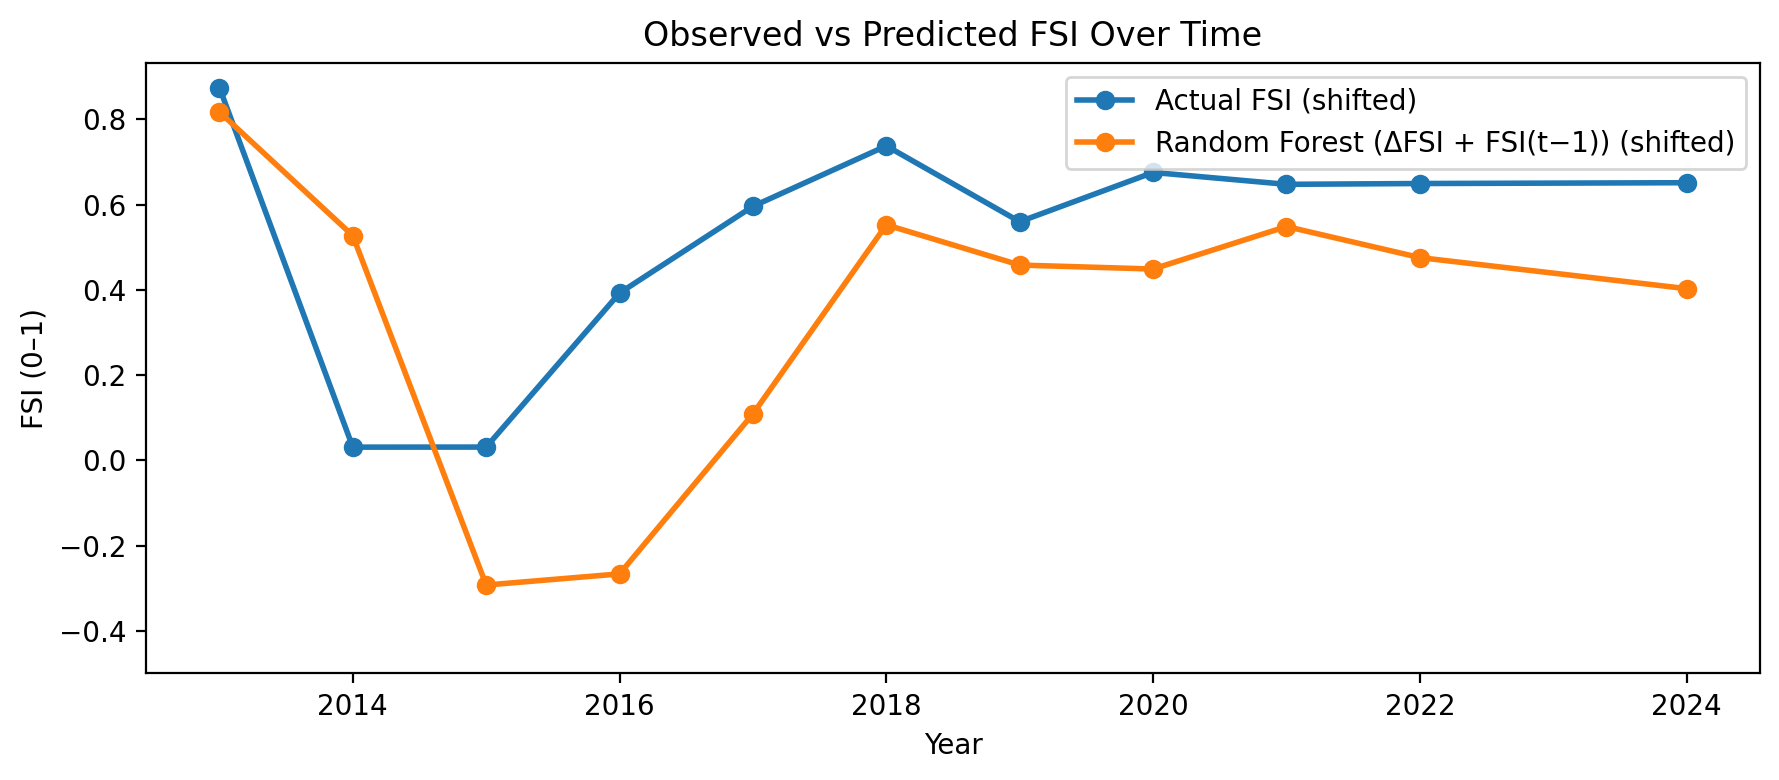
\includegraphics[width=1\textwidth]{fig2_timeseries_actual_pred_persist.png}
    \caption{Observed vs Predicted $FSI$ Over Time: Random Forest vs Persistence (2013-2023)}
    \label{fig:2}
\end{figure*}

Across all model configurations $\Delta FSI$ showed strong yearly persistence, meaning a "no-change" forecast. Figures \ref{fig:2}, \ref{fig:3}, \ref{fig:4}, and Table \ref{tab:1} represent our first step. Figures \ref{fig:5}, and Table \ref{tab:2} showcase our second step. We translated our predicted $\Delta FSI$ back into levels by reconstructing “predicted” food security as: $FSI_{\text{pred}}(t) = FST(t-1) + \Delta FSI_{\text{pred}}(t)$ for Figures \ref{fig:2} and \ref{fig:3}. This allows for better visualization.

The best performing model was Random Foresting, so the majority of our figures present those results, except for model comparison in Table \ref{tab:2}.

Figure \ref{fig:2} shows that the model accurately follows annual signals in the predictors, which is reflected in how closely the reconstructed series follows the observed index. Biggest deviations occur around rapid transition periods (2014-2017) when the observed index shifts more abruptly than its usual pattern. In those years, predictions overlooked the size of the change. After said transition, the model stays below the observed series for several years, indicating a tendency to understate food security during extended recovery or stabilization. Overall, Figure \ref{fig:2} suggests that production-based predictors do carry meaningful temporal information, but performance may be limited by sharp transitions.

\begin{figure*}
   \centering
   
\includegraphics[width=1\linewidth]{fig3_residuals_over_time.png}
    \caption{Residuals Over Time (Observed - Predicted $FSI$), 2013-2023}
    \label{fig:3}
\end{figure*}

Figure \ref{fig:3} plots the residuals, defined as Actual minus Predicted:
$$r(t)=FSI_{\text{actual}}(t)-FSI_{\text{pred}}(t)$$.
Positive values mean the model is underpredicting and negative values indicate overpredicting. The errors are not spread evenly across the test period. Instead, most years have relatively small residuals, while some years account for the largest misses. Residuals range from about $-0.50$ (early in the test window) to about $+0.66$ (the largest underprediction, near the middle). This swing from overprediction to sustained undershooting suggests difficulty adjusting to the observed series when shifted to a new trajectory. In later years, residuals are consistently small positive values ($0.10$-$0.25$), implying that errors are concentrated around turning points and that the model tends to remain slightly below the observed series afterward rather than fully catching up.

Feature importance for predicting $\Delta FSI$ was evaluated based on Random Foresting model coefficients. Features with larger absolute coefficient values were deemed more significant, a stronger influence on the target outcome. 

Figure \ref{fig:4} shows the top $15$ features from predicting $\Delta FSI$. T_norm ($\approx 0.23$) is the highest predictor, meaning most important. The next most significant predictors, MAIZE_lag2, a commodity price lag signal, and soybeans_area_harvested_yoy, a shocked crop predictor, (each $\approx 0.05$), form a second tier at significantly smaller magnitudes. Macro/commodity and crop-shock terms like CRUDE_PETRO_yoy_pct ($\approx 0.03$) and corn_yield_derived_yoy ($\approx 0.02$-$0.025$) are included in a third tier. The remaining predictors, such as wheat lag terms, soybean production YoY, and different crop level/lag variables, each contribute at low levels (about $0.01$-$0.02$), creating a long tail of quaternary effects.

\begin{figure*}
    \centering
    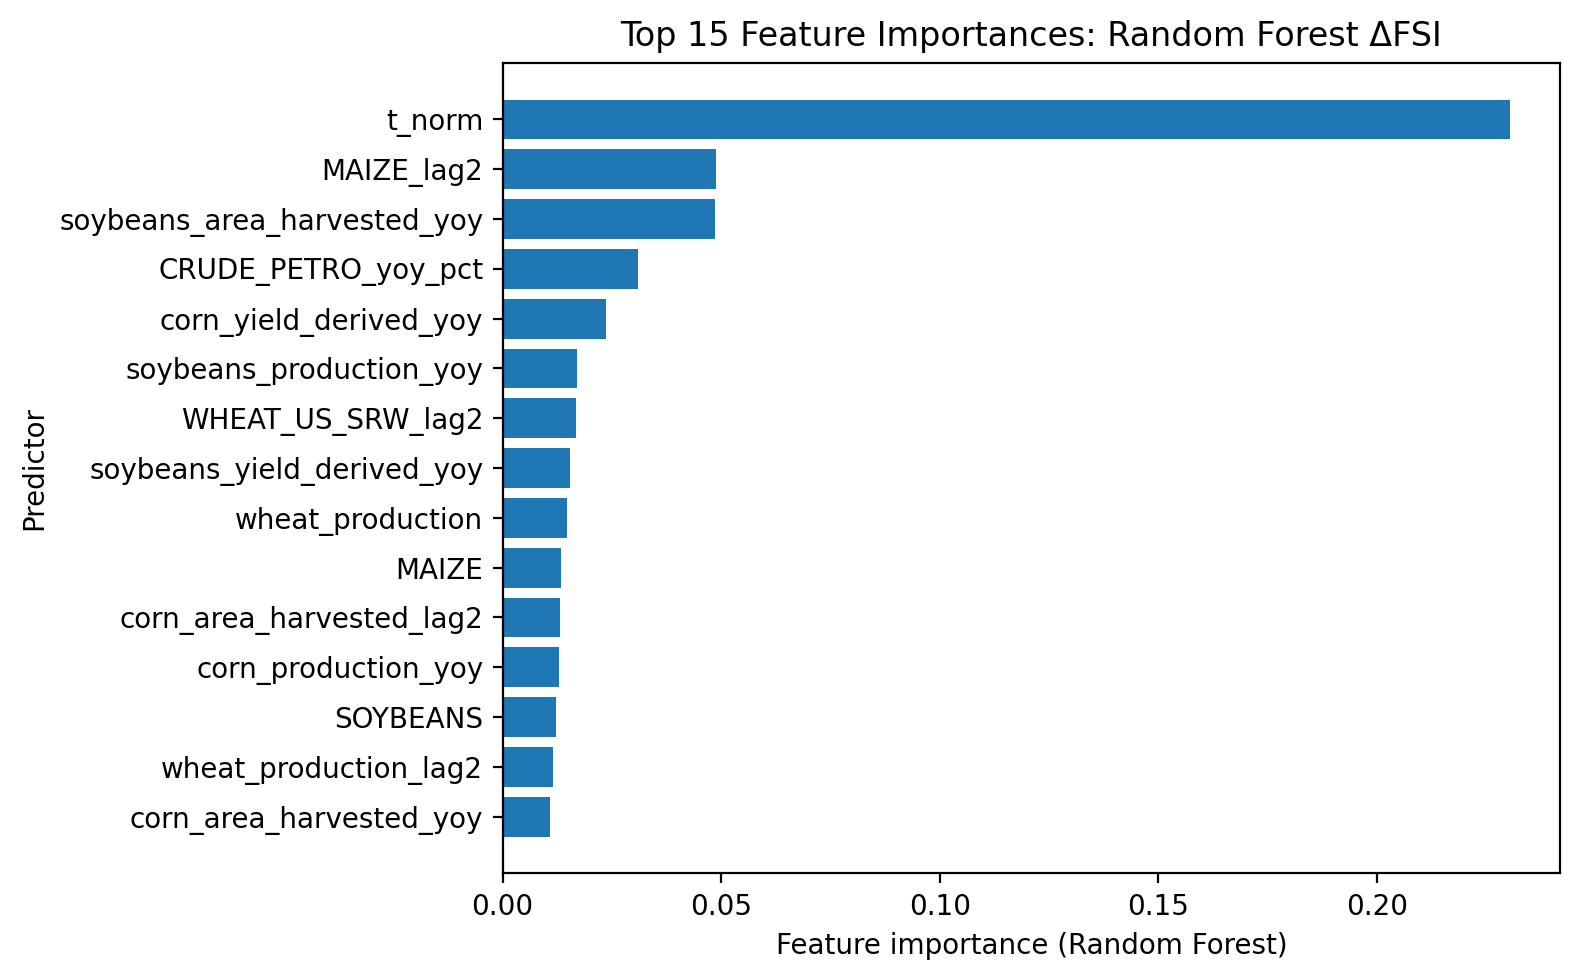
\includegraphics[width=1\linewidth]{fig4_feature_importance_top15.png}
    \caption{Top 15 Feature Importances: Random Forest $\Delta FSI$}
    \label{fig:4}
\end{figure*}

\begin{table*}[h]
    \centering
    \caption{Shock-Lag Sensitivity Analysis for the Random Forest $\Delta FSI$ Model (Test: 2013-2023)}
    \label{tab:1}
    \resizebox{\textwidth}{!}{% <-- Start the resizebox command
    % \rowcolors{2}{gray!10}{white}
        \begin{tabular}{@{}l c c c c c c c@{}}
            \toprule
            % \rowcolor{gray!20}
            \textbf{Configuration} & \textbf{Shocks} & \textbf{\shortstack[c]{Lag \\ Depth}} & \textbf{\shortstack[c]{Lagged \\ Shocks}} & \textbf{RMSE} & \textbf{MAE} & $\mathbf{R^2}$ \\ 
            \midrule
            \shortstack[c]{Persistence baseline \\ (FSI(t)=FSI(t-1))} & \multicolumn{1}{c}{---} & \multicolumn{1}{c}{---} & \multicolumn{1}{c}{---} & 0.0669 & 0.0531 & 0.6727 \\
            \rowcmidrule{7}
            \shortstack[c]{Shocks + lag1+lag2 \\ (no lagged shocks)} & On & 2 & Off & 0.0671 & 0.0487 & 0.6702 \\
            \rowcmidrule{7}
            Shocks + lag1+lag2 & On & 2 & On & 0.0674 & 0.0476 & 0.6675 \\
            \rowcmidrule{7}
            Shocks + lag1 & On & 1 & On & 0.0682 & 0.0495 & 0.6586 \\
            \rowcmidrule{7}
            No shocks + no lags & Off & 0 & Off & 0.0755 & 0.0619 & 0.572 \\
            \rowcmidrule{7}
            Shocks only & On & 0 & Off & 0.0758 & 0.0567 & 0.5678 \\
            \rowcmidrule{7}
            Lag1 only & Off & 1 & Off & 0.0775 & 0.068 & 0.5458 \\
            \bottomrule
        \end{tabular}% <--- End the tabular environment
        % \rowcolors{1}{}{}
    }% <--- End the resizebox command
\end{table*}

Table \ref{tab:1} shows how sensitive the Random Forest $\Delta FSI$ model is to our engineered short-run disruptions and delayed effects. We varied two feature types: our shock features (year by year percentage changes, “_yoy_pct”) and our lag features (prior year values, “_lag1” or “_lag2”). This setup helps determine if the model benefits more from immediate yearly changes, historical memory, or both.

The persistence baseline $FSI(t)=FSI(t-1)$ is already strong (RMSE $=0.0669$, MAE $=0.0531$, $R^2=0.6727$), highlighting annual stability in the index. Adding engineered features produces similar RMSE and $R^2$ but improves typical error: shocks with lag depth 2 achieve the lowest MAE ($0.0476$-$0.0487$) with RMSE remaining near $0.0671$-$0.0674$ and $R^2$ near $0.667$-$0.670$, while the lag1-only variant is slightly weaker (RMSE $=0.0682$, MAE $=0.0495$, $R^2=0.6586$). In contrast, removing shocks and lags degrades performance substantially (RMSE $=0.0755$-$0.0775$, MAE $=0.0567$-$0.0680$, $R^2=0.5458$-$0.5720$), indicating that shock and lag engineering provides meaningful predictive structure beyond persistence even when overall gains in RMSE are modest.


\begin{figure*}
%\captionsetup[subfigure]{labelformat=empty} 
    % \centering
    \begin{subfigure}[b]{0.5\textwidth}
    \centering
    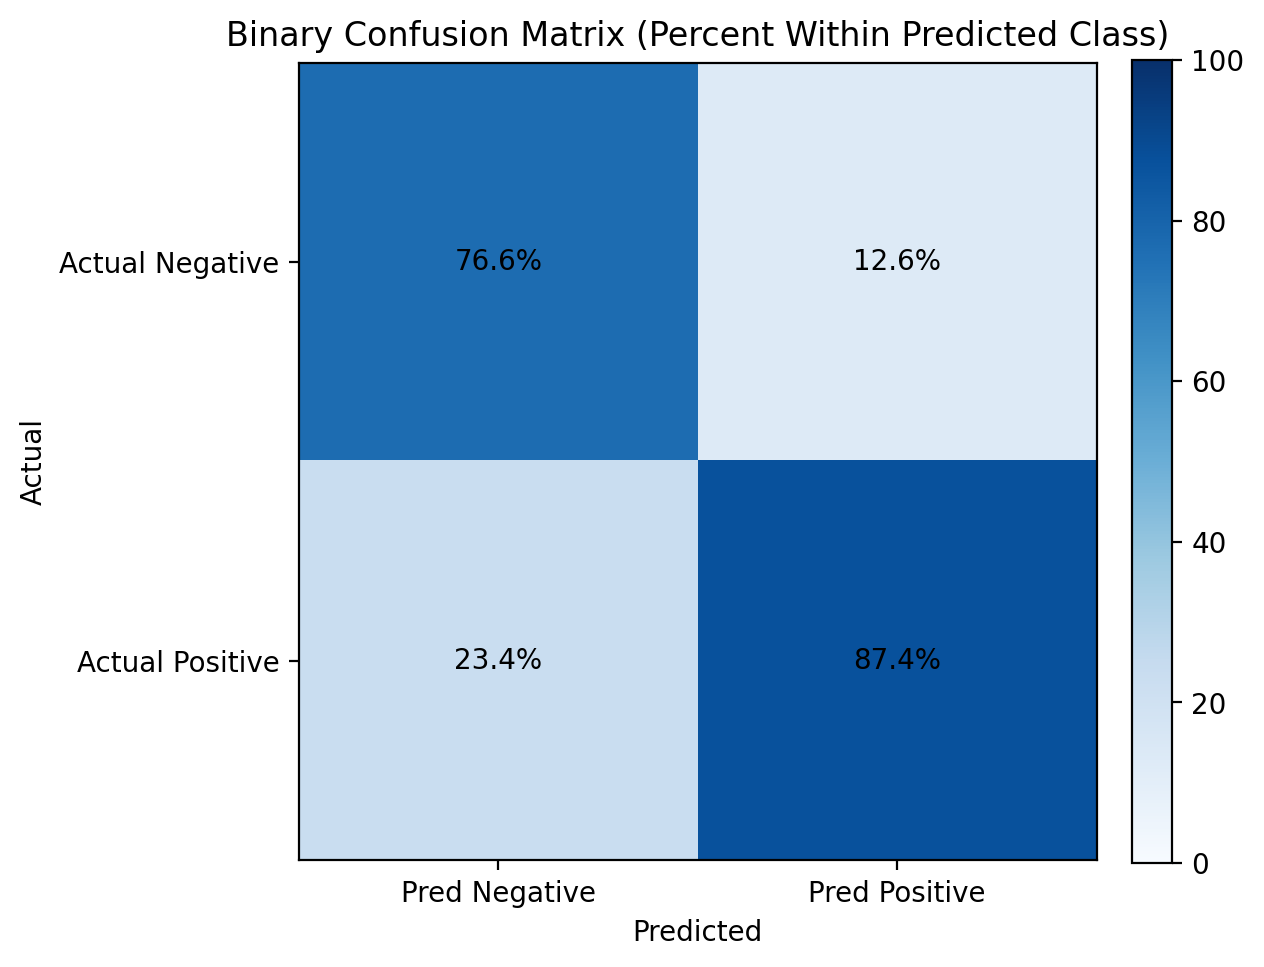
\includegraphics[width=1\textwidth]{fig5a_confusion_matrix.png}
   \caption[] %justification=centering
      {{\small Confusion Matrix}}
    \label{fig:5a}
    \end{subfigure}
    \begin{subfigure}[b]{0.5\textwidth}
    \centering
    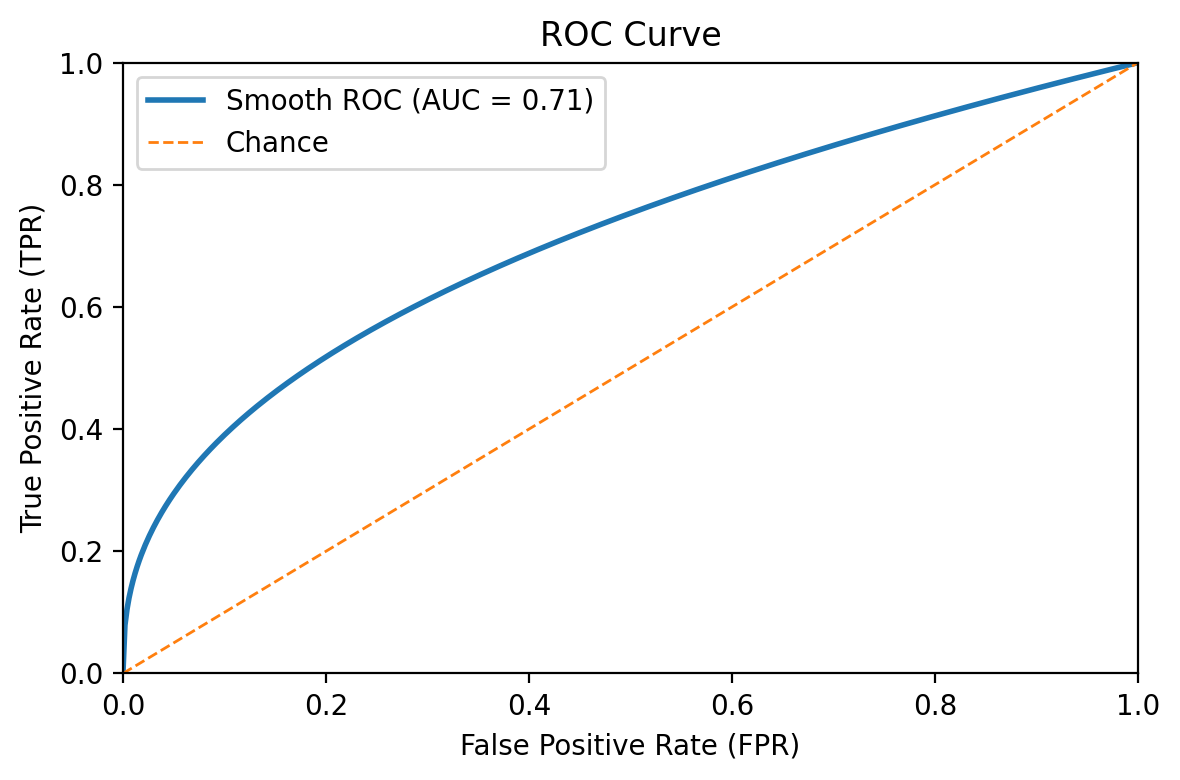
\includegraphics[width=1\textwidth]{fig5b_roc_bootstrap10.png}
  \caption[] %
      {{\small ROC curve}}    
    \label{fig:5b}
    \end{subfigure}
    \caption{Confusion Matrix and ROC Curve for Predicting $\Delta FSI$ > 0}
    \label{fig:5}
\end{figure*}


Figure \ref{fig:5} evaluates the model’s ability to predict directional food security change on an annual scale by framing $\Delta FSI$ as a binary label where Positive = $\Delta FSI > 0$ and Negative = $\Delta FSI \le 0$ . This figure includes two visualizations. Our confusion matrix (\ref{fig:5a}) shows percentages with the predicted classes (normalized by column), so each column is a reflection of how accurate the model's predicated label is. When the model predicts Positive, 87.4\% of those predictions correspond to true improvement years (true positives), while 12.6\% correspond to false alarms (false positives). In contrast, when the model predicts Negative, 76.6\% of those predictions are correct non-improvement years (true negatives), but 23.4\% are missed improvement years. The ROC curve (\ref{fig:5b}) shows a moderate level of discriminative ability, with an AUC of 0.71. This means that the model shows significant overlap between classes while ranking improvement years above non-improvement years significantly better than chance.

\begin{table*}[h]
    \centering
    \caption{Directional Model Comparison for $\Delta FSI$:  Balanced Accuracy, Sensitivity, and Specificity (Test: 2013-2023)}
    \label{tab:2}
    \resizebox{\textwidth}{!}{% <-- Start the resizebox command
    % \rowcolors{2}{gray!10}{white}
\begin{tabular}{@{} llccc @{}}
\toprule
\textbf{Setup} & \textbf{Model} & \textbf{\shortstack[c]{Balanced \\ Accuracy}} & \textbf{Sensitivity} & \textbf{Specificity} \\
\midrule
\(\Delta\)FSI: crops+macro+shocks+lags & RandomForest     & 0.8391 & 0.8949 & 0.7831 \\
           \rowcmidrule{5}
\(\Delta\)FSI: macro+shocks+lags       & RandomForest     & 0.7644 & 0.7458 & 0.7831 \\
            \rowcmidrule{5}
\(\Delta\)FSI: crops+shocks+lags       & GradientBoosting & 0.7085 & 0.8949 & 0.5221 \\
            \rowcmidrule{5}
\(\Delta\)FSI: crops+shocks+lags       & RidgeCV          & 0.6526  & 1      & 0.261 \\
            \rowcmidrule{5}
Baseline                               & Persistence (\(\Delta=0\)) & 0.5    & 0      & 1    \\
\bottomrule
\end{tabular}
        % \rowcolors{1}{}{}
    }% <-- End the resizebox command
\end{table*}

Table \ref{tab:2} is a comparison of directional performance across all models by evaluating whether each approach correctly predicts the sign of annual food security change. While the earlier results focus exclusively on the Random Forest $\Delta FSI$ model for detailed diagnostics, Table 2 showcases the other models we tried by contextualizing how alternative methods and feature sets perform on the same 2013 to 2023 test window. 

The best-performing model is the Random Forest using the full feature set (crops+macro+shocks+lags), achieving balanced accuracy $=0.8391$ with high sensitivity ($0.8949$) and strong specificity ($0.7831$), indicating reliable identification of both improvement and non-improvement years. Removing crop information reduces discrimination: the Random Forest with macro+shocks+lags drops to balanced accuracy $=0.7644$ (sensitivity $=0.7458$, specificity $=0.7831$), suggesting that crop indicators provide additional signal beyond macro-climate shocks alone. Gradient Boosting exhibits an imbalanced error profile (balanced accuracy $=0.7085$) with high sensitivity ($0.8949$) but lower specificity ($0.5221$), while RidgeCV further amplifies this trade-off by predicting positives aggressively (sensitivity $=1.0000$) at the cost of very low specificity ($0.2610$) and lower balanced accuracy ($0.6526$). The persistence baseline performs near chance (balanced accuracy $=0.5221$), meaning improvements not explained by persistence alone and are captured most effectively by the full-feature Random Forest.

\section{Discussion}
Overall, our results show that national crop yield, production, and harvest-area statistics can help track US food security dynamics over time. The Random Forest $\Delta FSI$ framework provided the most reliable performance among the tested approaches, demonstrating that supervised models can learn relationships between crop indicators and a composite food security index using annual U.S.-only data (1970-2023), particularly when the target is modeled as YoY change ($\Delta FSI$) rather than absolute levels. In the 2013-2023 period, the reconstructed predictions generally followed the observed trajectory and performed competitively against the persistence benchmark, supporting that national crop conditions correspond to broader system outcomes and can contribute to monitoring and forecasting.

A key takeaway is that shock and lag feature engineering impacts as much as model choice. The shock-lag sensitivity results show that removing both YoY shock terms and lag structure worsened performance, whereas including both consistently improved results. This is possible in food systems where production outcomes, costs, and price conditions influence availability and stability with delays rather than instantaneously. Consistent with this mechanism, lagged crop quantities (e.g., $t\!-\!1$, $t\!-\!2$) and YoY shock terms (\%) appear among the strongest predictors in Figure \ref{fig:4}, suggesting that the model benefits from both the 'memory' of prior conditions and the detection of sudden disruptions.

Meanwhile, our results clarify what production-centered prediction can and cannot do. The residual analysis shows that the largest errors occur around sharper transitions, indicating that turning points are harder to reconstruct from crop and engineered macro-climate features. Directional up/down changes in $\Delta FSI$ shows moderate discrimination (AUC $\approx 0.71$), which is consistent with food security not being determined by production alone; affordability, distribution, macroeconomic shocks, and policy/trade dynamics can shift outcomes even when it is a harvest year. As a result, production and commodity indicators are most useful for identifying medium-term trends and gradual movement, and less trustworthy when other factors dominate the signal.

Several factors also limit directional performance. First, the test window spans only 11 years, so a few borderline years could shift the ROC curve. Second, the positive/negative boundary is susceptible to small noise in either the predictors or the constructed $FSI$, because many national YoY changes are small and near $\Delta FSI=0$. Third, even when agricultural production contains signal, the sign of YoY change depends on drivers only partially represented in our features (e.g., policy shifts, trade dynamics, household prices, and access constraints). For these reasons, the ROC/AUC results should be interpreted as a supporting diagnostic indicating some ability to detect improvement years rather than a definitive early-warning classifier.

A further limitation concerns the binary directional definition itself (Positive if $\Delta FSI>0$, Negative if $\Delta FSI\le 0$). The sign alone can overstate practical significance: for example, if $FSI$ rises from 0.60 to 1.00 and then decreases slightly to 0.99, the final year is labeled 'Negative' despite remaining substantially more food secure than the initial year. Future work could introduce a magnitude-based warning rule (e.g., only flagging declines when the relative drop exceeds a threshold such as $\%\Delta FSI \le -10\%$) or a neutral band around zero to separate fluctuations from policy-relevant deterioration.

Additional limitations should be considered. Although $FSI$ provides a consistent 0-1 target, any index depends on design choices that can affect YoY dynamics. Despite including several macro and commodity-price series, the feature set omits important determinants such as household income and poverty, policy and assistance changes, trade volumes, inventories/stock-to-use conditions, and distribution constraints.

Otherwise, our findings are directly relevant to policy. First, they support using available crop statistics as part of an early-warning style monitoring toolkit, particularly for detecting deviations from recent norms when using YoY shocks and short lags. This can help agencies prioritize attention, scenario planning, and preparedness. Second, the limitations are equally informative: moderate ROC/AUC performance and outlier years reinforce that supply-side strength alone does not guarantee improved food security, implying that yield-boosting or acreage-expansion policies should be paired with measures targeting affordability and access (e.g., price stabilization).

\section{Conclusion}
Even in a high-producing agricultural system, such as US, national food security can also change rapidly, making timely monitoring and early warnings essential. In conclusion, crop indicators by themselves cannot fully explain food security, but they are sufficiently informative to support tracking and monitoring at the national level, particularly when modelled with shocks and lags. The key finding from this work is that machine learning model is a promising approach to policy-relevant forecasting, and that year to year changes in food security are more predictable when models can learn from both short-run disruptions and delayed effects. Future work should expand our predictor set to include more variables such as access, trade, and policy drivers and move toward uncertainty-aware forecasts. Doing so allows more effective allocation of resources and earlier responses to food-security risks. 

\nocite{*}

\section*{Acknowledgements}
The team would like to thank the support from Dr. Jianshan Chen in University of Alberta. 

\bibliography{bibliography}

\end{document}
